\section{Sub\-Bar\-Management Class Reference}
\label{classSubBarManagement}\index{SubBarManagement@{SubBarManagement}}
{\tt \#include $<$subbarmanagement.h$>$}

Inheritance diagram for Sub\-Bar\-Management:\begin{figure}[H]
\begin{center}
\leavevmode
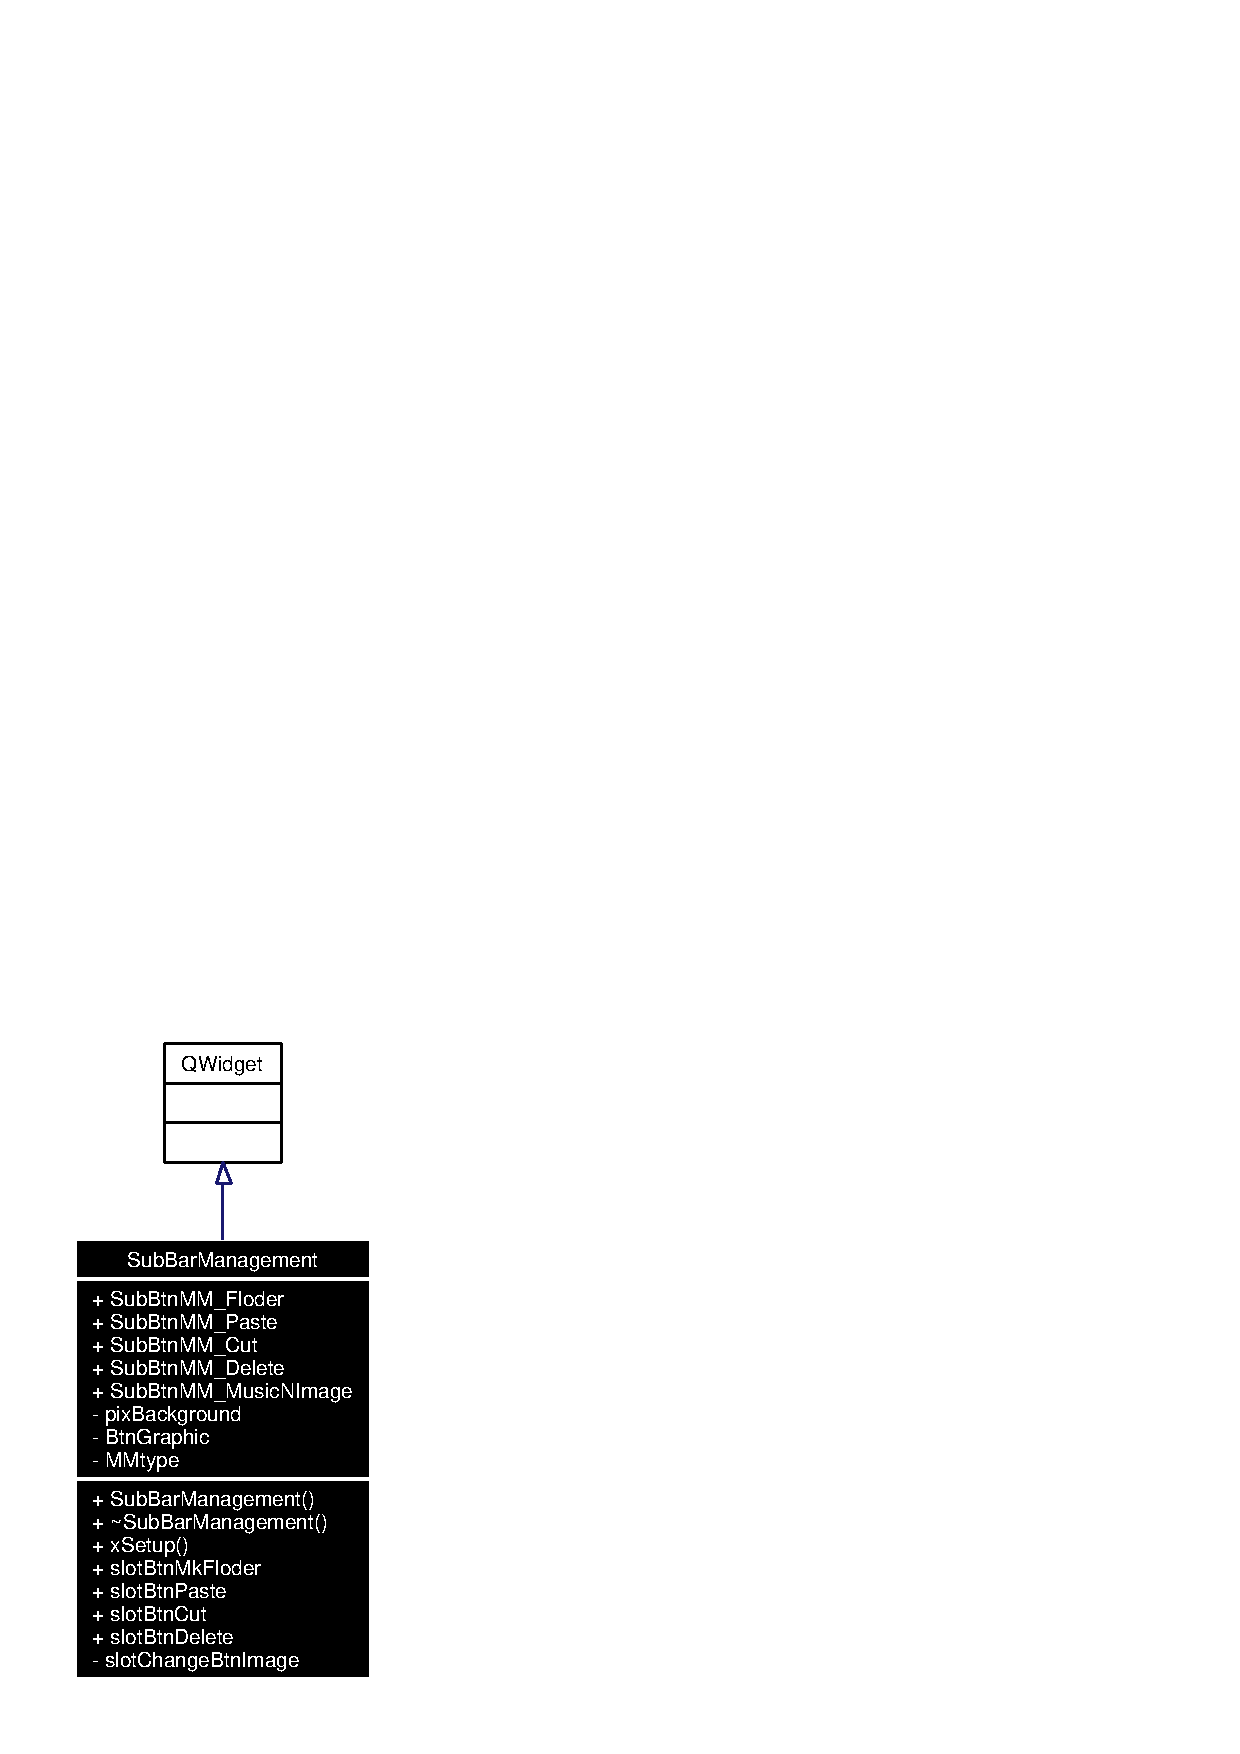
\includegraphics[width=89pt]{classSubBarManagement__inherit__graph}
\end{center}
\end{figure}
Collaboration diagram for Sub\-Bar\-Management:\begin{figure}[H]
\begin{center}
\leavevmode
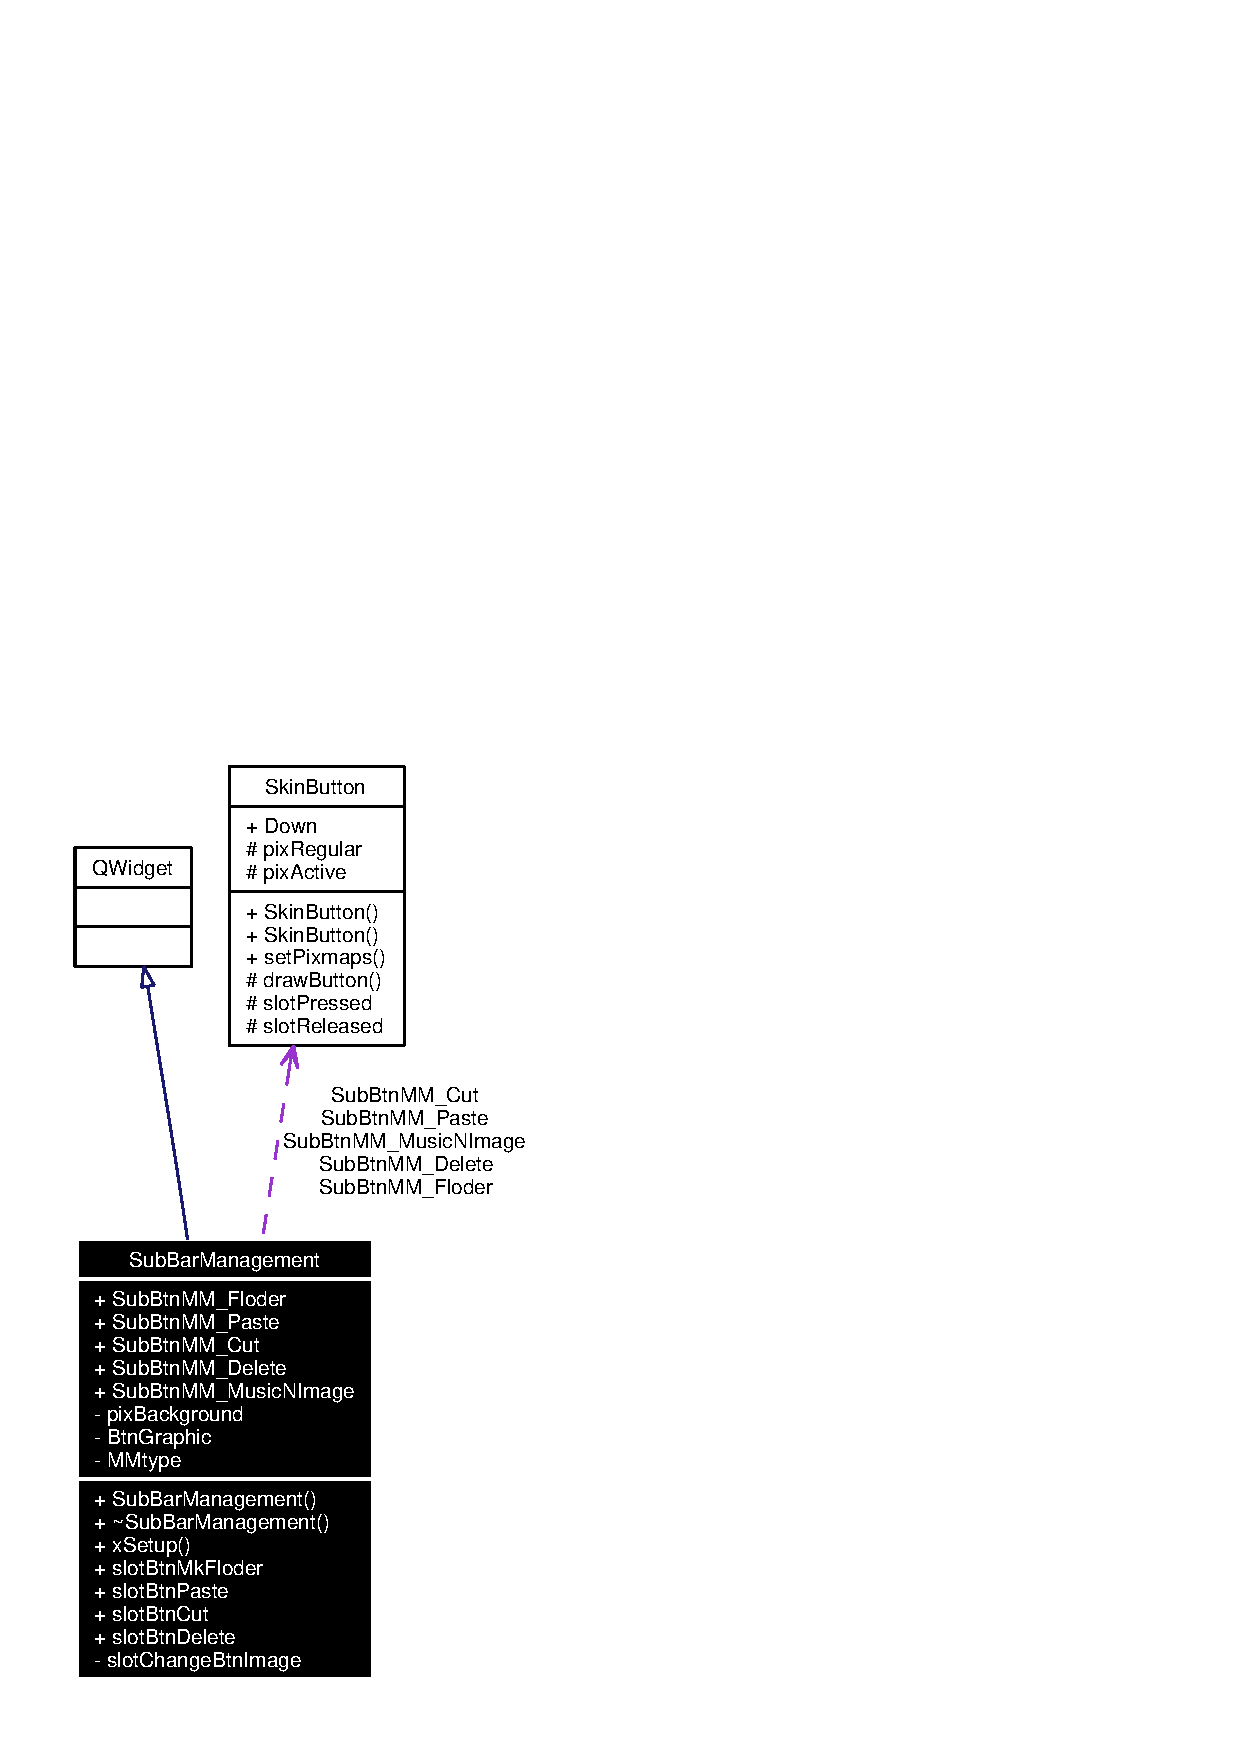
\includegraphics[width=135pt]{classSubBarManagement__coll__graph}
\end{center}
\end{figure}


\subsection{Detailed Description}
\begin{Desc}
\item[Author:]sonicat \end{Desc}




Definition at line 29 of file subbarmanagement.h.\subsection*{Public Slots}
\begin{CompactItemize}
\item 
void {\bf slot\-Btn\-Mk\-Floder} ()
\item 
void {\bf slot\-Btn\-Paste} ()
\item 
void {\bf slot\-Btn\-Cut} ()
\item 
void {\bf slot\-Btn\-Delete} ()
\end{CompactItemize}
\subsection*{Signals}
\begin{CompactItemize}
\item 
void {\bf signal\-Management\-Mode\-Change} (int)
\item 
void {\bf signal\-Mkdir} ()
\item 
void {\bf singal\-Paste\-FUNC\_\-MEDIAM} ()
\item 
void {\bf signal\-Cut\-FUNC\_\-MEDIAM} ()
\item 
void {\bf signal\-Delete\-Item} ()
\end{CompactItemize}
\subsection*{Public Member Functions}
\begin{CompactItemize}
\item 
{\bf Sub\-Bar\-Management} ({\bf QWidget} $\ast$parent=0, const char $\ast$name=0)
\item 
{\bf $\sim$Sub\-Bar\-Management} ()
\item 
void {\bf x\-Setup} ()
\end{CompactItemize}
\subsection*{Public Attributes}
\begin{CompactItemize}
\item 
{\bf Skin\-Button} $\ast$ {\bf Sub\-Btn\-MM\_\-Floder}
\item 
{\bf Skin\-Button} $\ast$ {\bf Sub\-Btn\-MM\_\-Paste}
\item 
{\bf Skin\-Button} $\ast$ {\bf Sub\-Btn\-MM\_\-Cut}
\item 
{\bf Skin\-Button} $\ast$ {\bf Sub\-Btn\-MM\_\-Delete}
\item 
{\bf Skin\-Button} $\ast$ {\bf Sub\-Btn\-MM\_\-Music\-NImage}
\end{CompactItemize}
\subsection*{Private Types}
\begin{CompactItemize}
\item 
enum {\bf MM\_\-TYPE} \{ {\bf em\_\-mmimage}, 
{\bf em\_\-mmmusic}
 \}
\end{CompactItemize}
\subsection*{Private Slots}
\begin{CompactItemize}
\item 
void {\bf slot\-Change\-Btn\-Image} ()
\end{CompactItemize}
\subsection*{Private Attributes}
\begin{CompactItemize}
\item 
QPixmap {\bf pix\-Background}
\item 
QPixmap $\ast$ {\bf Btn\-Graphic} [12]
\item 
{\bf MM\_\-TYPE} {\bf MMtype}
\end{CompactItemize}


\subsection{Member Enumeration Documentation}
\index{SubBarManagement@{Sub\-Bar\-Management}!MM_TYPE@{MM\_\-TYPE}}
\index{MM_TYPE@{MM\_\-TYPE}!SubBarManagement@{Sub\-Bar\-Management}}
\subsubsection{\setlength{\rightskip}{0pt plus 5cm}enum {\bf Sub\-Bar\-Management::MM\_\-TYPE}\hspace{0.3cm}{\tt  [private]}}\label{classSubBarManagement_SubBarManagementy2}


\begin{Desc}
\item[Enumeration values: ]\par
\begin{description}
\index{em_mmimage@{em\_\-mmimage}!SubBarManagement@{SubBarManagement}}\index{SubBarManagement@{SubBarManagement}!em_mmimage@{em\_\-mmimage}}\item[{\em 
em\_\-mmimage\label{classSubBarManagement_SubBarManagementy2SubBarManagementy0}
}]\index{em_mmmusic@{em\_\-mmmusic}!SubBarManagement@{SubBarManagement}}\index{SubBarManagement@{SubBarManagement}!em_mmmusic@{em\_\-mmmusic}}\item[{\em 
em\_\-mmmusic\label{classSubBarManagement_SubBarManagementy2SubBarManagementy1}
}]\end{description}
\end{Desc}



Definition at line 32 of file subbarmanagement.h.



\footnotesize\begin{verbatim}32 {em_mmimage,em_mmmusic};
\end{verbatim}\normalsize 


\subsection{Constructor \& Destructor Documentation}
\index{SubBarManagement@{Sub\-Bar\-Management}!SubBarManagement@{SubBarManagement}}
\index{SubBarManagement@{SubBarManagement}!SubBarManagement@{Sub\-Bar\-Management}}
\subsubsection{\setlength{\rightskip}{0pt plus 5cm}Sub\-Bar\-Management::Sub\-Bar\-Management ({\bf QWidget} $\ast$ {\em parent} = 0, const char $\ast$ {\em name} = 0)}\label{classSubBarManagement_SubBarManagementa0}




Definition at line 22 of file subbarmanagement.cpp.

References x\-Setup().



\footnotesize\begin{verbatim}23  : QWidget(parent, name)
24 {
25   xSetup();
26 }
\end{verbatim}\normalsize 


Here is the call graph for this function:\begin{figure}[H]
\begin{center}
\leavevmode
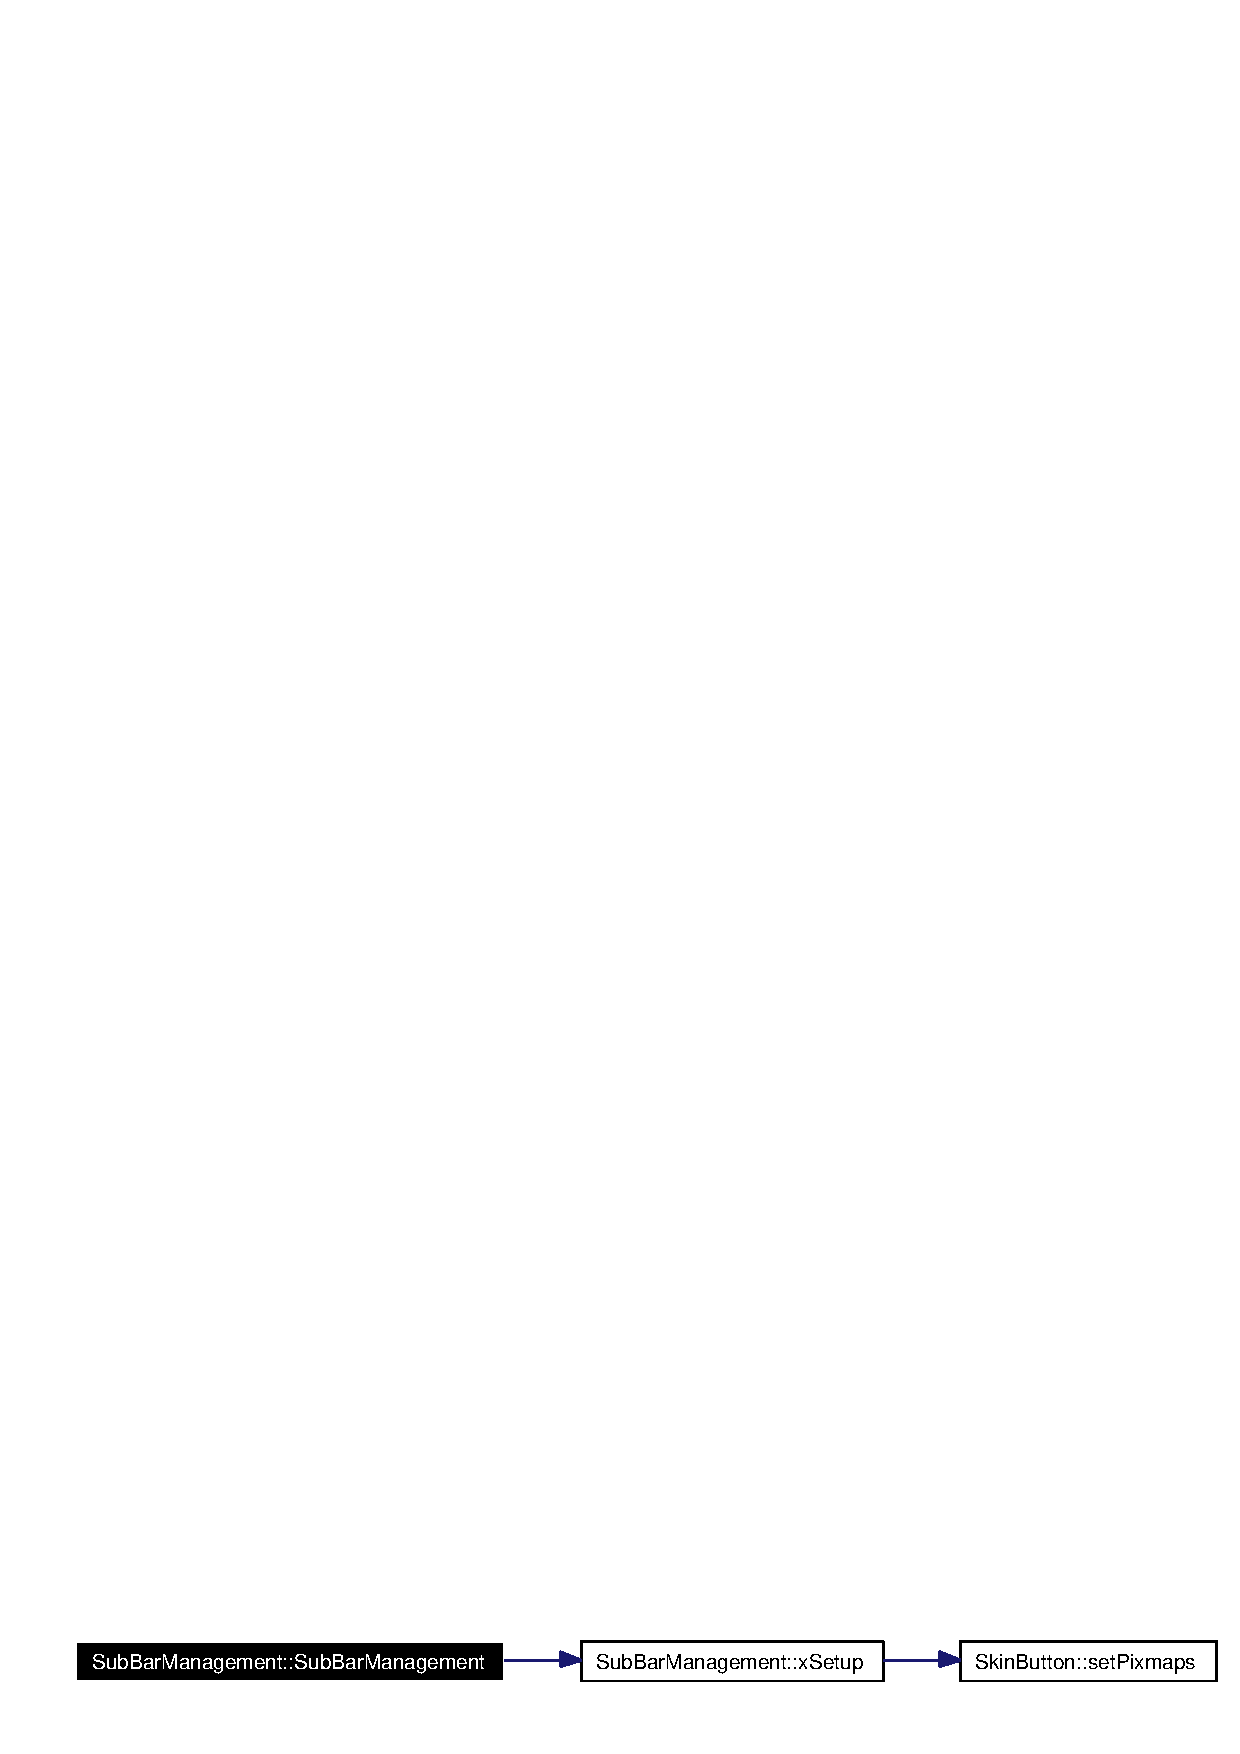
\includegraphics[width=292pt]{classSubBarManagement_SubBarManagementa0_cgraph}
\end{center}
\end{figure}
\index{SubBarManagement@{Sub\-Bar\-Management}!~SubBarManagement@{$\sim$SubBarManagement}}
\index{~SubBarManagement@{$\sim$SubBarManagement}!SubBarManagement@{Sub\-Bar\-Management}}
\subsubsection{\setlength{\rightskip}{0pt plus 5cm}Sub\-Bar\-Management::$\sim${\bf Sub\-Bar\-Management} ()}\label{classSubBarManagement_SubBarManagementa1}




Definition at line 29 of file subbarmanagement.cpp.



\footnotesize\begin{verbatim}30 {
31 }
\end{verbatim}\normalsize 


\subsection{Member Function Documentation}
\index{SubBarManagement@{Sub\-Bar\-Management}!signalCutFUNC_MEDIAM@{signalCutFUNC\_\-MEDIAM}}
\index{signalCutFUNC_MEDIAM@{signalCutFUNC\_\-MEDIAM}!SubBarManagement@{Sub\-Bar\-Management}}
\subsubsection{\setlength{\rightskip}{0pt plus 5cm}void Sub\-Bar\-Management::signal\-Cut\-FUNC\_\-MEDIAM ()\hspace{0.3cm}{\tt  [signal]}}\label{classSubBarManagement_SubBarManagementl3}




Definition at line 121 of file subbarmanagement.moc.

Referenced by slot\-Btn\-Cut().



\footnotesize\begin{verbatim}122 {
123     activate_signal( staticMetaObject()->signalOffset() + 3 );
124 }
\end{verbatim}\normalsize 
\index{SubBarManagement@{Sub\-Bar\-Management}!signalDeleteItem@{signalDeleteItem}}
\index{signalDeleteItem@{signalDeleteItem}!SubBarManagement@{Sub\-Bar\-Management}}
\subsubsection{\setlength{\rightskip}{0pt plus 5cm}void Sub\-Bar\-Management::signal\-Delete\-Item ()\hspace{0.3cm}{\tt  [signal]}}\label{classSubBarManagement_SubBarManagementl4}




Definition at line 127 of file subbarmanagement.moc.

Referenced by slot\-Btn\-Delete().



\footnotesize\begin{verbatim}128 {
129     activate_signal( staticMetaObject()->signalOffset() + 4 );
130 }
\end{verbatim}\normalsize 
\index{SubBarManagement@{Sub\-Bar\-Management}!signalManagementModeChange@{signalManagementModeChange}}
\index{signalManagementModeChange@{signalManagementModeChange}!SubBarManagement@{Sub\-Bar\-Management}}
\subsubsection{\setlength{\rightskip}{0pt plus 5cm}void Sub\-Bar\-Management::signal\-Management\-Mode\-Change (int)\hspace{0.3cm}{\tt  [signal]}}\label{classSubBarManagement_SubBarManagementl0}




Definition at line 103 of file subbarmanagement.moc.

Referenced by slot\-Change\-Btn\-Image().



\footnotesize\begin{verbatim}104 {
105     activate_signal( staticMetaObject()->signalOffset() + 0, t0 );
106 }
\end{verbatim}\normalsize 
\index{SubBarManagement@{Sub\-Bar\-Management}!signalMkdir@{signalMkdir}}
\index{signalMkdir@{signalMkdir}!SubBarManagement@{Sub\-Bar\-Management}}
\subsubsection{\setlength{\rightskip}{0pt plus 5cm}void Sub\-Bar\-Management::signal\-Mkdir ()\hspace{0.3cm}{\tt  [signal]}}\label{classSubBarManagement_SubBarManagementl1}




Definition at line 109 of file subbarmanagement.moc.

Referenced by slot\-Btn\-Mk\-Floder().



\footnotesize\begin{verbatim}110 {
111     activate_signal( staticMetaObject()->signalOffset() + 1 );
112 }
\end{verbatim}\normalsize 
\index{SubBarManagement@{Sub\-Bar\-Management}!singalPasteFUNC_MEDIAM@{singalPasteFUNC\_\-MEDIAM}}
\index{singalPasteFUNC_MEDIAM@{singalPasteFUNC\_\-MEDIAM}!SubBarManagement@{Sub\-Bar\-Management}}
\subsubsection{\setlength{\rightskip}{0pt plus 5cm}void Sub\-Bar\-Management::singal\-Paste\-FUNC\_\-MEDIAM ()\hspace{0.3cm}{\tt  [signal]}}\label{classSubBarManagement_SubBarManagementl2}




Definition at line 115 of file subbarmanagement.moc.

Referenced by slot\-Btn\-Paste().



\footnotesize\begin{verbatim}116 {
117     activate_signal( staticMetaObject()->signalOffset() + 2 );
118 }
\end{verbatim}\normalsize 
\index{SubBarManagement@{Sub\-Bar\-Management}!slotBtnCut@{slotBtnCut}}
\index{slotBtnCut@{slotBtnCut}!SubBarManagement@{Sub\-Bar\-Management}}
\subsubsection{\setlength{\rightskip}{0pt plus 5cm}void Sub\-Bar\-Management::slot\-Btn\-Cut ()\hspace{0.3cm}{\tt  [slot]}}\label{classSubBarManagement_SubBarManagementi2}




Definition at line 115 of file subbarmanagement.cpp.

References signal\-Cut\-FUNC\_\-MEDIAM().

Referenced by x\-Setup().



\footnotesize\begin{verbatim}116 {
117   emit signalCutFUNC_MEDIAM();
118 }
\end{verbatim}\normalsize 
\index{SubBarManagement@{Sub\-Bar\-Management}!slotBtnDelete@{slotBtnDelete}}
\index{slotBtnDelete@{slotBtnDelete}!SubBarManagement@{Sub\-Bar\-Management}}
\subsubsection{\setlength{\rightskip}{0pt plus 5cm}void Sub\-Bar\-Management::slot\-Btn\-Delete ()\hspace{0.3cm}{\tt  [slot]}}\label{classSubBarManagement_SubBarManagementi3}




Definition at line 120 of file subbarmanagement.cpp.

References signal\-Delete\-Item().

Referenced by x\-Setup().



\footnotesize\begin{verbatim}121 {
122   emit signalDeleteItem();
123 }
\end{verbatim}\normalsize 
\index{SubBarManagement@{Sub\-Bar\-Management}!slotBtnMkFloder@{slotBtnMkFloder}}
\index{slotBtnMkFloder@{slotBtnMkFloder}!SubBarManagement@{Sub\-Bar\-Management}}
\subsubsection{\setlength{\rightskip}{0pt plus 5cm}void Sub\-Bar\-Management::slot\-Btn\-Mk\-Floder ()\hspace{0.3cm}{\tt  [slot]}}\label{classSubBarManagement_SubBarManagementi0}




Definition at line 105 of file subbarmanagement.cpp.

References signal\-Mkdir().

Referenced by x\-Setup().



\footnotesize\begin{verbatim}106 {
107   emit signalMkdir();
108 }
\end{verbatim}\normalsize 
\index{SubBarManagement@{Sub\-Bar\-Management}!slotBtnPaste@{slotBtnPaste}}
\index{slotBtnPaste@{slotBtnPaste}!SubBarManagement@{Sub\-Bar\-Management}}
\subsubsection{\setlength{\rightskip}{0pt plus 5cm}void Sub\-Bar\-Management::slot\-Btn\-Paste ()\hspace{0.3cm}{\tt  [slot]}}\label{classSubBarManagement_SubBarManagementi1}




Definition at line 110 of file subbarmanagement.cpp.

References singal\-Paste\-FUNC\_\-MEDIAM().

Referenced by x\-Setup().



\footnotesize\begin{verbatim}111 {
112   emit singalPasteFUNC_MEDIAM();
113 }
\end{verbatim}\normalsize 
\index{SubBarManagement@{Sub\-Bar\-Management}!slotChangeBtnImage@{slotChangeBtnImage}}
\index{slotChangeBtnImage@{slotChangeBtnImage}!SubBarManagement@{Sub\-Bar\-Management}}
\subsubsection{\setlength{\rightskip}{0pt plus 5cm}void Sub\-Bar\-Management::slot\-Change\-Btn\-Image ()\hspace{0.3cm}{\tt  [private, slot]}}\label{classSubBarManagement_SubBarManagementk0}




Definition at line 89 of file subbarmanagement.cpp.

References em\_\-mmimage, em\_\-mmmusic, MMtype, Skin\-Button::set\-Pixmaps(), signal\-Management\-Mode\-Change(), and Sub\-Btn\-MM\_\-Music\-NImage.

Referenced by x\-Setup().



\footnotesize\begin{verbatim}90 {
91    if(MMtype==em_mmmusic)
92    {
93       MMtype=em_mmimage;
94       SubBtnMM_MusicNImage->setPixmaps(BtnGraphic[10],BtnGraphic[11]);
95       emit signalManagementModeChange(0);
96    }
97    else
98    {
99      MMtype=em_mmmusic;
100      SubBtnMM_MusicNImage->setPixmaps(BtnGraphic[8],BtnGraphic[9]);
101      emit signalManagementModeChange(1);
102    }
103 }
\end{verbatim}\normalsize 
\index{SubBarManagement@{Sub\-Bar\-Management}!xSetup@{xSetup}}
\index{xSetup@{xSetup}!SubBarManagement@{Sub\-Bar\-Management}}
\subsubsection{\setlength{\rightskip}{0pt plus 5cm}void Sub\-Bar\-Management::x\-Setup ()}\label{classSubBarManagement_SubBarManagementa2}




Definition at line 33 of file subbarmanagement.cpp.

References em\_\-mmmusic, MMtype, Skin\-Button::set\-Pixmaps(), slot\-Btn\-Cut(), slot\-Btn\-Delete(), slot\-Btn\-Mk\-Floder(), slot\-Btn\-Paste(), slot\-Change\-Btn\-Image(), Sub\-Btn\-MM\_\-Cut, Sub\-Btn\-MM\_\-Delete, Sub\-Btn\-MM\_\-Floder, Sub\-Btn\-MM\_\-Music\-NImage, and Sub\-Btn\-MM\_\-Paste.

Referenced by Sub\-Bar\-Management().



\footnotesize\begin{verbatim}34 {
35    //DAVID Setup Background;
36    pixBackground.load("/root/kde_application/hdass08/skin/SubBarBackground.png");
37    setBackgroundPixmap(pixBackground);
38    
39    //DAVID init state
40    MMtype=em_mmmusic;
41    
42    //Btn Graphic
43    BtnGraphic[0]=new QPixmap("/root/kde_application/hdass08/skin/Bar-MM-Btn-Floder.png");
44    BtnGraphic[1]=new QPixmap("/root/kde_application/hdass08/skin/Bar-MM-Btn-Floder-Active.png");
45    BtnGraphic[2]=new QPixmap("/root/kde_application/hdass08/skin/Bar-MM-Btn-Paste.png");
46    BtnGraphic[3]=new QPixmap("/root/kde_application/hdass08/skin/Bar-MM-Btn-Paste-Active.png");
47    BtnGraphic[4]=new QPixmap("/root/kde_application/hdass08/skin/Bar-MM-Btn-Cut.png");
48    BtnGraphic[5]=new QPixmap("/root/kde_application/hdass08/skin/Bar-MM-Btn-Cut-Active.png");
49    BtnGraphic[6]=new QPixmap("/root/kde_application/hdass08/skin/Bar-MM-Btn-Delete.png");
50    BtnGraphic[7]=new QPixmap("/root/kde_application/hdass08/skin/Bar-MM-Btn-Delete-Active.png");
51    BtnGraphic[8]=new QPixmap("/root/kde_application/hdass08/skin/Bar-MM-Btn-Music.png");
52    BtnGraphic[9]=new QPixmap("/root/kde_application/hdass08/skin/Bar-MM-Btn-Music-Active.png");
53    BtnGraphic[10]=new QPixmap("/root/kde_application/hdass08/skin/Bar-MM-Btn-Image.png");
54    BtnGraphic[11]=new QPixmap("/root/kde_application/hdass08/skin/Bar-MM-Btn-Image-Active.png");
55    
56    SubBtnMM_Floder=new SkinButton(this);
57    SubBtnMM_Paste=new SkinButton(this);
58    SubBtnMM_Cut=new SkinButton(this);
59    SubBtnMM_Delete=new SkinButton(this);
60    SubBtnMM_MusicNImage=new SkinButton(this);
61    
62    SubBtnMM_Floder->setPixmaps(BtnGraphic[0],BtnGraphic[1]);
63    SubBtnMM_Floder->setGeometry(197,0,60,80);
64    SubBtnMM_Floder->show();
65    
66    SubBtnMM_Paste->setPixmaps(BtnGraphic[2],BtnGraphic[3]);
67    SubBtnMM_Paste->setGeometry(263,0,60,80);
68    SubBtnMM_Paste->show();
69    
70    SubBtnMM_Cut->setPixmaps(BtnGraphic[4],BtnGraphic[5]);
71    SubBtnMM_Cut->setGeometry(329,0,60,80);
72    SubBtnMM_Cut->show();
73    
74    SubBtnMM_Delete->setPixmaps(BtnGraphic[6],BtnGraphic[7]);
75    SubBtnMM_Delete->setGeometry(391,0,60,80);
76    SubBtnMM_Delete->show();
77    
78    SubBtnMM_MusicNImage->setPixmaps(BtnGraphic[8],BtnGraphic[9]);
79    SubBtnMM_MusicNImage->setGeometry(457,0,80,80);
80    SubBtnMM_MusicNImage->show();
81    
82    //DAVID Connect buttons
83    QObject::connect(SubBtnMM_MusicNImage,SIGNAL(pressed()),this,SLOT(slotChangeBtnImage()));
84    QObject::connect(SubBtnMM_Floder,SIGNAL(pressed()),this,SLOT(slotBtnMkFloder()));
85    QObject::connect(SubBtnMM_Paste,SIGNAL(pressed()),this,SLOT(slotBtnPaste()));
86    QObject::connect(SubBtnMM_Cut,SIGNAL(pressed()),this,SLOT(slotBtnCut()));
87    QObject::connect(SubBtnMM_Delete ,SIGNAL(pressed()),this,SLOT(slotBtnDelete()));
88 }
\end{verbatim}\normalsize 


Here is the call graph for this function:\begin{figure}[H]
\begin{center}
\leavevmode
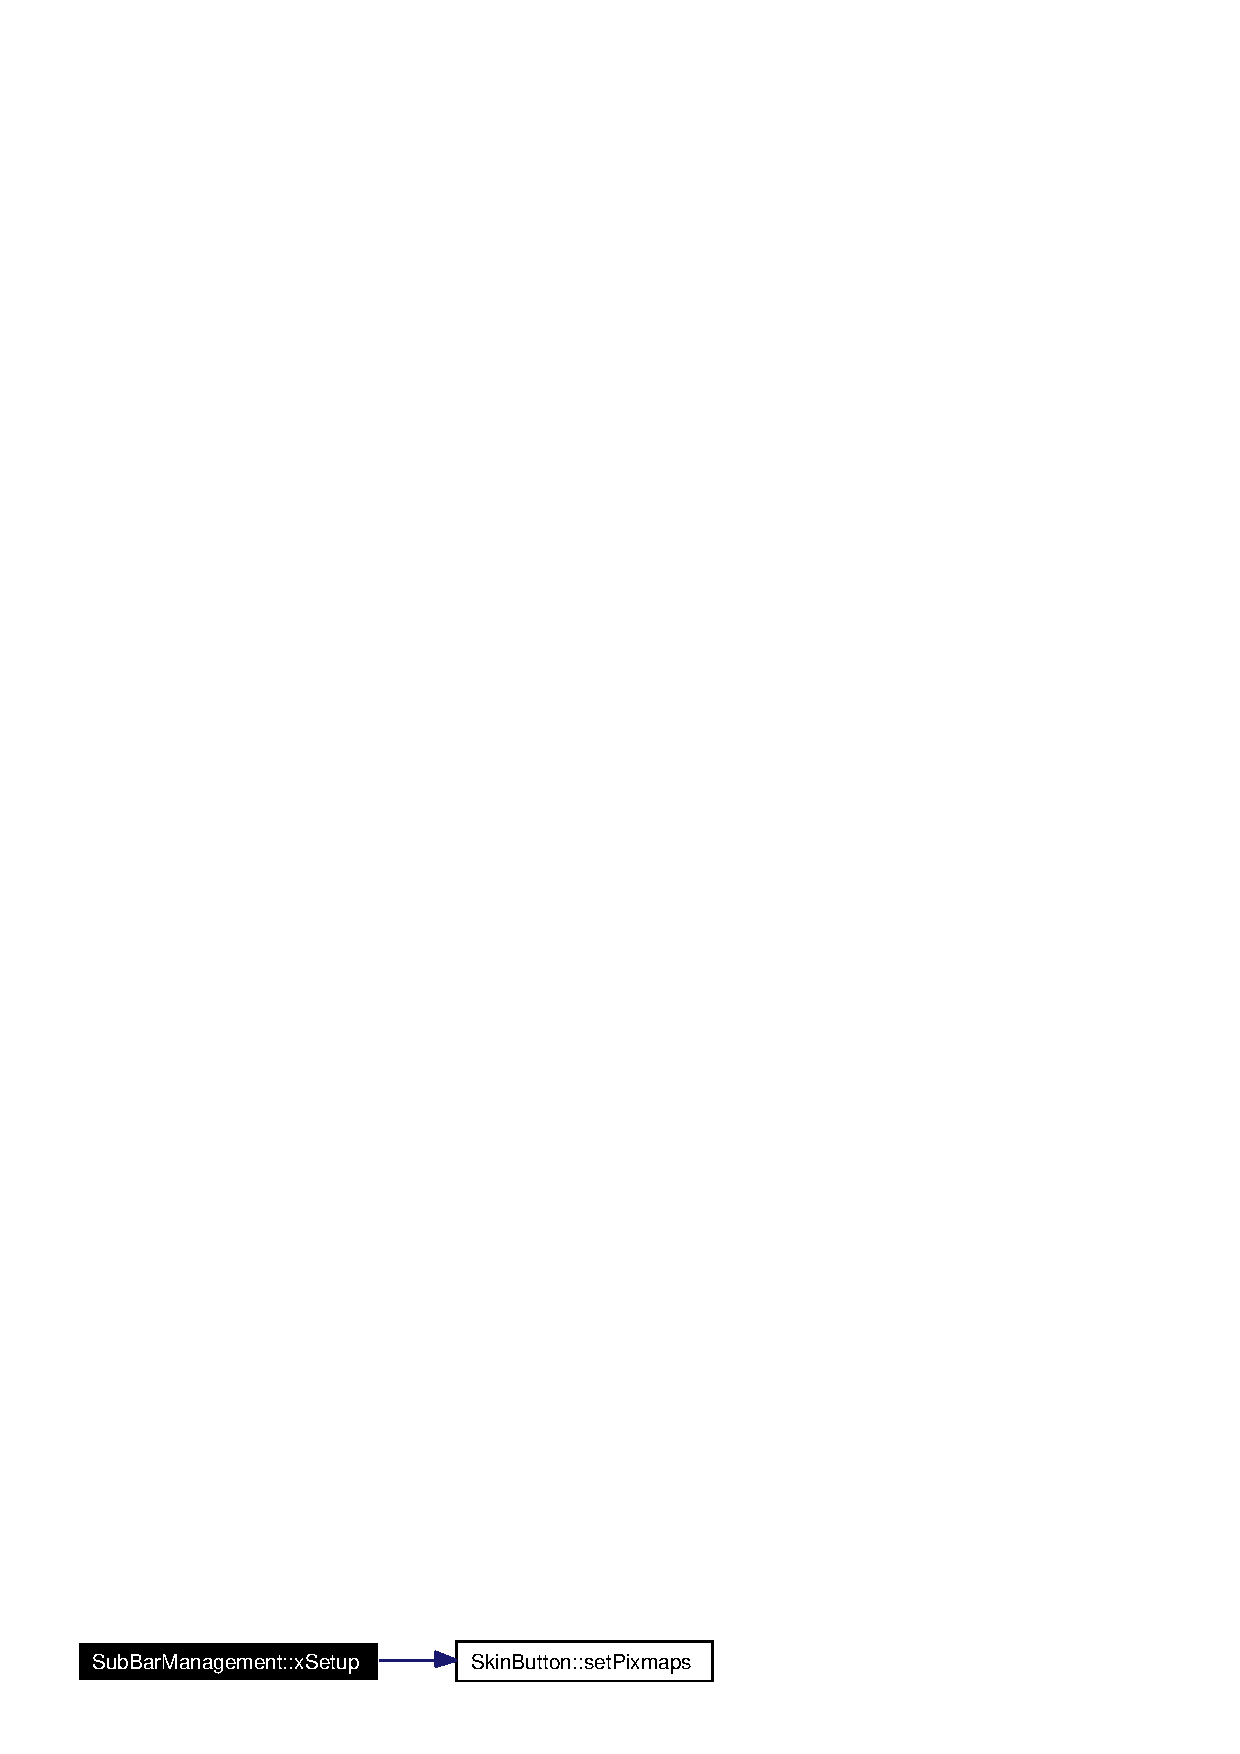
\includegraphics[width=171pt]{classSubBarManagement_SubBarManagementa2_cgraph}
\end{center}
\end{figure}


\subsection{Member Data Documentation}
\index{SubBarManagement@{Sub\-Bar\-Management}!BtnGraphic@{BtnGraphic}}
\index{BtnGraphic@{BtnGraphic}!SubBarManagement@{Sub\-Bar\-Management}}
\subsubsection{\setlength{\rightskip}{0pt plus 5cm}QPixmap$\ast$ {\bf Sub\-Bar\-Management::Btn\-Graphic}[12]\hspace{0.3cm}{\tt  [private]}}\label{classSubBarManagement_SubBarManagementr1}




Definition at line 54 of file subbarmanagement.h.\index{SubBarManagement@{Sub\-Bar\-Management}!MMtype@{MMtype}}
\index{MMtype@{MMtype}!SubBarManagement@{Sub\-Bar\-Management}}
\subsubsection{\setlength{\rightskip}{0pt plus 5cm}{\bf MM\_\-TYPE} {\bf Sub\-Bar\-Management::MMtype}\hspace{0.3cm}{\tt  [private]}}\label{classSubBarManagement_SubBarManagementr2}




Definition at line 55 of file subbarmanagement.h.

Referenced by slot\-Change\-Btn\-Image(), and x\-Setup().\index{SubBarManagement@{Sub\-Bar\-Management}!pixBackground@{pixBackground}}
\index{pixBackground@{pixBackground}!SubBarManagement@{Sub\-Bar\-Management}}
\subsubsection{\setlength{\rightskip}{0pt plus 5cm}QPixmap {\bf Sub\-Bar\-Management::pix\-Background}\hspace{0.3cm}{\tt  [private]}}\label{classSubBarManagement_SubBarManagementr0}




Definition at line 53 of file subbarmanagement.h.\index{SubBarManagement@{Sub\-Bar\-Management}!SubBtnMM_Cut@{SubBtnMM\_\-Cut}}
\index{SubBtnMM_Cut@{SubBtnMM\_\-Cut}!SubBarManagement@{Sub\-Bar\-Management}}
\subsubsection{\setlength{\rightskip}{0pt plus 5cm}{\bf Skin\-Button} $\ast$ {\bf Sub\-Bar\-Management::Sub\-Btn\-MM\_\-Cut}}\label{classSubBarManagement_SubBarManagemento2}




Definition at line 38 of file subbarmanagement.h.

Referenced by x\-Setup().\index{SubBarManagement@{Sub\-Bar\-Management}!SubBtnMM_Delete@{SubBtnMM\_\-Delete}}
\index{SubBtnMM_Delete@{SubBtnMM\_\-Delete}!SubBarManagement@{Sub\-Bar\-Management}}
\subsubsection{\setlength{\rightskip}{0pt plus 5cm}{\bf Skin\-Button} $\ast$ {\bf Sub\-Bar\-Management::Sub\-Btn\-MM\_\-Delete}}\label{classSubBarManagement_SubBarManagemento3}




Definition at line 38 of file subbarmanagement.h.

Referenced by x\-Setup().\index{SubBarManagement@{Sub\-Bar\-Management}!SubBtnMM_Floder@{SubBtnMM\_\-Floder}}
\index{SubBtnMM_Floder@{SubBtnMM\_\-Floder}!SubBarManagement@{Sub\-Bar\-Management}}
\subsubsection{\setlength{\rightskip}{0pt plus 5cm}{\bf Skin\-Button}$\ast$ {\bf Sub\-Bar\-Management::Sub\-Btn\-MM\_\-Floder}}\label{classSubBarManagement_SubBarManagemento0}




Definition at line 38 of file subbarmanagement.h.

Referenced by x\-Setup().\index{SubBarManagement@{Sub\-Bar\-Management}!SubBtnMM_MusicNImage@{SubBtnMM\_\-MusicNImage}}
\index{SubBtnMM_MusicNImage@{SubBtnMM\_\-MusicNImage}!SubBarManagement@{Sub\-Bar\-Management}}
\subsubsection{\setlength{\rightskip}{0pt plus 5cm}{\bf Skin\-Button} $\ast$ {\bf Sub\-Bar\-Management::Sub\-Btn\-MM\_\-Music\-NImage}}\label{classSubBarManagement_SubBarManagemento4}




Definition at line 38 of file subbarmanagement.h.

Referenced by slot\-Change\-Btn\-Image(), and x\-Setup().\index{SubBarManagement@{Sub\-Bar\-Management}!SubBtnMM_Paste@{SubBtnMM\_\-Paste}}
\index{SubBtnMM_Paste@{SubBtnMM\_\-Paste}!SubBarManagement@{Sub\-Bar\-Management}}
\subsubsection{\setlength{\rightskip}{0pt plus 5cm}{\bf Skin\-Button} $\ast$ {\bf Sub\-Bar\-Management::Sub\-Btn\-MM\_\-Paste}}\label{classSubBarManagement_SubBarManagemento1}




Definition at line 38 of file subbarmanagement.h.

Referenced by x\-Setup().

The documentation for this class was generated from the following files:\begin{CompactItemize}
\item 
{\bf subbarmanagement.h}\item 
{\bf subbarmanagement.moc}\item 
{\bf subbarmanagement.cpp}\end{CompactItemize}
